\documentclass[12pt,oneside]{uhthesis}
\usepackage{subfigure}
\usepackage[ruled,lined,linesnumbered,titlenumbered,algochapter,spanish,onelanguage]{algorithm2e}
\usepackage{amsmath}
\usepackage{amssymb}
\usepackage{amsbsy}
\usepackage{caption,booktabs}
\captionsetup{ justification = centering }
%\usepackage{mathpazo}
\usepackage{float}
\setlength{\marginparwidth}{2cm}
\usepackage{todonotes}
\usepackage{listings}
\usepackage{xcolor}
\usepackage{multicol}
\usepackage{graphicx}
\floatstyle{plaintop}
\restylefloat{table}
\addbibresource{Bibliography.bib}
% \setlength{\parskip}{\baselineskip}%
\renewcommand{\tablename}{Tabla}
\renewcommand{\listalgorithmcfname}{Índice de Algoritmos}
%\dontprintsemicolon
\SetAlgoNoEnd

\definecolor{codegreen}{rgb}{0,0.6,0}
\definecolor{codegray}{rgb}{0.5,0.5,0.5}
\definecolor{codepurple}{rgb}{0.58,0,0.82}
\definecolor{backcolour}{rgb}{0.95,0.95,0.92}

\lstdefinestyle{mystyle}{
    backgroundcolor=\color{backcolour},   
    commentstyle=\color{codegreen},
    keywordstyle=\color{purple},
    numberstyle=\tiny\color{codegray},
    stringstyle=\color{codepurple},
    basicstyle=\ttfamily\footnotesize,
    breakatwhitespace=false,         
    breaklines=true,                 
    captionpos=b,                    
    keepspaces=true,                 
    numbers=left,                    
    numbersep=5pt,                  
    showspaces=false,                
    showstringspaces=false,
    showtabs=false,                  
    tabsize=4
}

\lstset{style=mystyle}

\title{Título de la tesis}
\author{\\\vspace{0.25cm}Deborah Famadas Rodríguez}
\advisor{\\\vspace{0.25cm}Dr. Reinaldo Rodríguez Ramos,\\\vspace{0.2cm}Dr. Esteban Clua , Instituto de Computación, Universidad Federal Fluminense de Rio de Janeiro}
\degree{Licenciado en Ciencia de la Computación}
\faculty{Facultad de Matemática y Computación}
\date{Fecha\\\vspace{0.25cm}\href{https://github.com/username/repo}{github.com/username/repo}}
\logo{Graphics/uhlogo}
\makenomenclature

\renewcommand{\vec}[1]{\boldsymbol{#1}}
\newcommand{\diff}[1]{\ensuremath{\mathrm{d}#1}}
\newcommand{\me}[1]{\mathrm{e}^{#1}}
\newcommand{\pf}{\mathfrak{p}}
\newcommand{\qf}{\mathfrak{q}}
%\newcommand{\kf}{\mathfrak{k}}
\newcommand{\kt}{\mathtt{k}}
\newcommand{\mf}{\mathfrak{m}}
\newcommand{\hf}{\mathfrak{h}}
\newcommand{\fac}{\mathrm{fac}}
\newcommand{\maxx}[1]{\max\left\{ #1 \right\} }
\newcommand{\minn}[1]{\min\left\{ #1 \right\} }
\newcommand{\lldpcf}{1.25}
\newcommand{\nnorm}[1]{\left\lvert #1 \right\rvert }
\renewcommand{\lstlistingname}{Ejemplo de código}
\renewcommand{\lstlistlistingname}{Ejemplos de código}

\begin{document}

\frontmatter
\maketitle

\begin{dedication}
    Dedicación
\end{dedication}
\begin{acknowledgements}
    Agradecimientos
\end{acknowledgements}
\begin{opinion}
    Opiniones de los tutores
\end{opinion}
\begin{resumen}
	El Machine Learning (ML) o Aprendizaje Automático (AM) es un subcampo de la Inteligencia Artificial (IA),
que se define como la capacidad de una máquina para aprender, mejorando su rendimiento. Los avances en
las tecnologías de IA y ML prometen. El potencial de estas herramientas para generar conocimiento a partir de cantidades masivas
de datos es enorme, pudiendo así ayudar a tomar decisiones, que incluirán intervenciones, y tratamientos
de precisión contra el cáncer. La detección de cáncer de piel utilizando Redes Neuronales Convolucionales (CNN) 
es un área prometedora en el campo de la inteligencia artificial y el aprendizaje automático. Las CNN son especialmente
adecuadas para el procesamiento de imágenes y han demostrado un alto rendimiento en tareas de clasificación y detección
de objetos. Este trabajo de diploma presenta una serie de implementaciones, las que incluyen CNN, el modelo EfficientNetB5 
y el uso de Learning Rate Adjustment a un Dataset de imágenes para lograr una detección efectiva de diferentes tipos de cáncer 
de piel a partir del entrenamiento de una IA. Estos resultados pueden sentar las bases para futuras investigaciones y mejoras 
en el campo de la detección temprana del cáncer de piel utilizando técnicas de aprendizaje automático y 
redes neuronales convolucionales.
\end{resumen}

\begin{abstract}
	Machine Learning (ML) or Machine Learning (ML) is a subfield of Artificial Intelligence (AI), which is defined 
as the ability of a machine to learn, improving its performance. Advances in AI and ML technologies hold promise. 
The potential of these tools to generate knowledge from massive amounts of data is enormous, thus being able to help 
make decisions, which will include interventions, and precision in cancer treatments. The detection of skin cancer using 
Convolutional Neural Networks (CNN)  is a promising area in the field of artificial intelligence and machine learning. 
CNNs are particularly well suited for image suitable for image processing and have demonstrated high performance in object 
classification and object detection tasks. This diploma work presents a number of implementations, which 
include CNNs, the EfficientNetB5 model, and the use of Learning Rate Adjustment to an image dataset to achieve 
effective detection of different types of skin cancer by training an from the training of an AI. These results can lay 
the foundation for future research and improvements in the field of early skin cancer detection using machine learning 
techniques.
\end{abstract}
\tableofcontents
\listoffigures
% \listoftables
% \listofalgorithms
\lstlistoflistings

\mainmatter

\chapter*{Introducción}\label{chapter:introduction}
\addcontentsline{toc}{chapter}{Introducción}

La medicina es una rama de la ciencia en constante evolución. Cada vez se desarrollan más métodos innovadores para mejorar el diagnóstico precoz 
de enfermedades potencialmente mortales cuya detección temprana puede prolongar considerablemente la esperanza de vida de los pacientes. En la actualidad, 
la detección del cáncer de piel es un proceso estrictamente humano que depende del oncólogo y de una prueba que en algunos países puede resultar cara 
(biopsia), aunque en algunos países ya se está intentando utilizar modelos computacionales para la detección.

La inteligencia artificial (IA) y el aprendizaje automático (ML) han experimentado un progreso significativo en los últimos años, y su aplicación 
en la detección de enfermedades, como el cáncer de piel, ha generado un gran interés en la comunidad científica. El ML y la IA han demostrado ser 
herramientas valiosas en la biología y la medicina, ayudando a los científicos a determinar fármacos potencialmente mejores y a entender de manera 
más profunda el comportamiento de la vida celular.

El avance en la detección de cáncer mediante el uso de la inteligencia artificial (IA) y el aprendizaje automático (ML) ha sido significativo en 
las últimas décadas. A continuación, se presenta una cronología de cómo ha ido avanzando la detección de cáncer con ML:

\begin{enumerate}
    \item 2016: Se publicaron estudios sobre el uso de modelos de ML para la predicción del sobrevivencia del cáncer de mama. \cite{ml-breast-cancer}
    \item 2018: Se realizaron investigaciones sobre el uso de técnicas de ML en el análisis de imágenes médicas para el diagnóstico y tratamiento de 
    diferentes tipos de cáncer, incluido el cáncer de piel. \cite{ml-cancer-pred-diag}
    \item 2022: Se publicaron revisiones sobre la aplicación de enfoques de ML en la segmentación y clasificación de lesiones de piel en imágenes 
    dermoscopicas. \cite{ml-techniques-review}
    \item 2023: Se publicaron estudios sobre el uso de la IA y el ML en la predicción de la respuesta a la inmunoterapia en el cáncer de pulmón.\cite{ai-lung-cancer}
\end{enumerate}

Al utilizar ML en la detección de cáncer de piel, se puede acelerar el proceso de diagnóstico, lo que permite a los médicos tomar decisiones de 
tratamiento más rápidas y efectivas nature.com. Esto es especialmente importante en el cáncer de piel, ya que la detección temprana y el tratamiento 
temprano pueden mejorar significativamente las perspectivas de supervivencia y calidad de vida de los pacientes.

La dermatología y la oncologic pueden acercarse a la informática a través de la detección precoz de afecciones cancerosas de la piel, con una foto de
una lesión en una fase temprana y un conjunto de datos de imágenes de lesiones diagnosticadas, 
más tarde, el ordenador puede ser entrenado para alertar a los médicos de posibles afecciones antes de que se desarrollen y se conviertan en letales.

Según la Sociedad Americana del Cáncer, Mitchell et al. (2020) \cite{mitchell}, los cánceres de piel melanoma tienen un estadio temprano 
formalmente llamado estadio 0 o melanoma \textit{in situ} donde el tratamiento arroja una tasa de éxito de casi el 100\% ya que sólo se necesita una 
cirugía menor para extirpar la porción de piel afectada. Esto hace que la detección precoz de esta enfermedad sea una premisa para mejorar el 
tratamiento oncológico.

Las enfermedades de la piel entrenadas para el modelo son las siguientes: Melanoma (MEL), Nevus Melanocítico (NV), Carcinoma de Células Basales (BCC), 
Queratosis Actínica, Enfermedad de Bowen (carcinoma intraepitelial) (AKIEC), Queratosis Benigna (BKL), Dermatofibroma (DF), Lesión Vascular (VASC).

\begin{enumerate} 
    \item[.] Melanoma (MEL): Es una forma agresiva de cáncer de piel que puede afectar a personas de cualquier edad. Se detecta mediante la observación de cambios 
    en las manchas de la piel, como nuevos crecimientos, cambios en el tamaño, forma o color, o sangrado. 
    \item[.] Nevus Melanocítico (NV): Son manchas de piel de color oscuro que pueden ser benignas o precursoras de cáncer de piel. Se detectan mediante la 
    observación de cambios en la piel, como nuevas manchas o cambios en el tamaño, forma o color de las manchas existentes.. 
    \item[.] Carcinoma de Células Basales (BCC): Es un tipo de cáncer de piel que generalmente se encuentra en áreas expuestas a la luz solar. Se detecta mediante 
    la observación de cambios en la piel, como nuevos crecimientos, cambios en el tamaño, forma o color, o la aparición de cicatrices de escamas.
    \item[.] Queratosis Actínica: Es una enfermedad de la piel que se caracteriza por la aparición de manchas de color rojizo a anaranjado en la piel. Se detecta 
    mediante la observación de cambios en la piel, como la aparición de nuevas manchas o cambios en el tamaño, forma o color de las manchas existentes. 
    y características que indiquen la presencia de queratosis actínica.
    \item[.] Enfermedad de Bowen (carcinoma intraepitelial) (AKIEC): Es un tipo de cáncer de piel que afecta a las capas superficiales de la piel. Se detecta mediante 
    la observación de cambios en la piel, como la aparición de nuevas manchas, cambios en el tamaño, forma o color de las manchas existentes, o la aparición 
    de cicatrices de escamas.
    \item[.] Queratosis Benigna (BKL): Es una enfermedad de la piel que se caracteriza por la aparición de manchas de color blanco en la piel. Se detecta mediante 
    la observación de cambios en la piel, como la aparición de nuevas manchas o cambios en el tamaño, forma o color de las manchas existentes.
    \item[.] Dermatofibroma (DF): Es una enfermedad de la piel que se caracteriza por la aparición de manchas de color blanco en la piel. Se detecta mediante la 
    observación de cambios en la piel, como la aparición de nuevas manchas o cambios en el tamaño, forma o color de las manchas existentes link.springer.com. 
    \item[.] Lesión Vascular (VASC): Son creencias de la piel causadas por enfermedades cutanosas. Se detecta mediante la observación de cambios en la piel, como 
    la aparición de nuevas manchas o cambios en el tamaño, forma o color de las manchas existentes.
\end{enumerate}

Para la deteccion mediante imagenes de los mencionados canceres de piel se utilizan Redes Neuronales Convolucionales para procesamiento de imágenes 
específicamente del tipo EfficientNetB5, así como métodos de aprendizaje supervisado, tales como, Support Vector Machine (SVM) y Learning Rate Adjustment
(LRA). Los datos utilizados corresponden al concurso HAM10000 (Human Against Machine, con 10000 imágenes de entrenamiento), que contiene imágenes 
dermatoscópicas de múltiples fuentes de lesiones cutáneas cancerosas y no cancerosas. Estas imágenes fueron previamente segmentadas, parametrizadas y 
clasificadas.Este aprendizaje automático puede ofrecer a la detección de diferentes tipos de cáncer en un primer momento. 

\chapter{Estado del Arte}\label{chapter:state-of-the-art}

\section{Modelo de aprendizaje automático basado en EfficientNetB5 para el diagnóstico de afecciones dermatológicas}\label{sec:dev}
%-----------------------------------------------------------------------------------
En este trabajo revisamos diferentes modelos de Machine Learning, los implementamos y proponemos parámetros y configuraciones enfocados al diagnóstico de afecciones dermatológicas. 
Nuestro modelo comienza procesando las imágenes a través de una Red Neuronal Convolucional, que entrega los resultados a una Máquina de Vectores Soporte que procederá a la clasificación de las imágenes segmentadas. 
Aplicamos una red EfficientNet a través de parámetros de tasa de aprendizaje sugeridos. A continuación detallamos cada una de las etapas. 

%-----------------------------------------------------------------------------------
	\subsection{Redes neuronales convolucionales}\label{sub:cnn}
%-----------------------------------------------------------------------------------
Las redes neuronales convolucionales (CNN) tienen una arquitectura específica que resulta especialmente útil en tareas de reconocimiento y clasificación de imágenes, como la identificación de caras, objetos y señales de tráfico. 
Las CNN se basan en métodos de aprendizaje supervisado, lo que significa que necesitan datos etiquetados para entrenarse. 
El objetivo principal es aprender la relación entre los objetos de entrada y sus correspondientes etiquetas de clase. 
Las CNN constan de dos componentes principales: las capas ocultas, que extraen características de los datos de entrada, y las capas totalmente conectadas, que realizan la tarea de clasificación propiamente dicha.

En comparación con las redes neuronales normales, la arquitectura de las capas ocultas de una CNN es única. 
En una red neuronal típica, cada capa contiene un conjunto de neuronas y cada neurona está conectada a todas las neuronas de la capa anterior. 
En una CNN, sin embargo, las neuronas de una capa sólo están conectadas a un pequeño número de neuronas de la capa anterior. 
Esto se debe a que las CNN se basan en operaciones de convolución, que consisten en filtrar una imagen utilizando una máscara. 
La salida de cada píxel es una combinación lineal de los píxeles de entrada. 
La entrada de una CNN suele ser una imagen con una anchura, una altura y un número de canales (W x H x D). 
El uso de convoluciones reduce la carga computacional del sistema, y esta restricción a conexiones locales y capas de agrupamiento simplifica el entrenamiento y reduce la complejidad del modelo.

%-----------------------------------------------------------------------------------
	\subsection{Máquina de vectores soporte (SVM)}\label{sub:svm}
%-----------------------------------------------------------------------------------
SVM (Support Vector Machine) es un enfoque supervisado que utiliza un algoritmo de aprendizaje principalmente para clasificar los datos en diferentes clases con el uso de un hiperplano que actúa como límite de decisión. 
La SVM estudia los datos de entrenamiento etiquetados y, a continuación, clasifica cualquier entrada nueva basándose en lo aprendido en la fase de entrenamiento. 
Se crea un hiperplano aleatorio y, a continuación, se comprueba la distancia entre el hiperplano y los puntos de datos más cercanos de cada clase. 
Estos puntos de datos más cercanos al hiperplano se conocen como vectores de soporte Y de ahí viene el nombre, máquinas de vectores de soporte.

En este proyecto SVM se utiliza para clasificar tumores malignos e imágenes benignas de cáncer de piel, esto se hace pasando las imágenes segmentadas y las características extraídas a SVM donde SVM escribe el hiperplano y agrupa todas las características cercanas similares en diferentes clases.

%-----------------------------------------------------------------------------------
	\subsection{Modelo EfficientNetB5}\label{sub:efficientnetB5}
%-----------------------------------------------------------------------------------
Las redes neuronales convolucionales %\cite{cnn} 
suelen desarrollarse con un coste fijo de recursos, y luego se escalan para lograr una mayor precisión cuando se dispone de más recursos. 
Por ejemplo, ResNet puede escalarse de ResNet-18 a ResNet-200 aumentando el número de capas.

La práctica convencional para escalar el modelo consiste en aumentar arbitrariamente la profundidad o la anchura de las redes neuronales convolucionales, o en utilizar una mayor resolución de la imagen de entrada para el entrenamiento y la evaluación. 
Aunque estos métodos mejoran la precisión, suelen requerir un tedioso ajuste manual y, aun así, a menudo producen un rendimiento subóptimo.
En concreto, EfficientNetB5 %\cite{tan} 
es una extensión de EfficientNetB0 \- B6 que se ajusta al tamaño de las imágenes que manejamos dentro del conjunto de datos.

%-----------------------------------------------------------------------------------
	\subsection{Learning Rate Adjustment (LRA)}\label{sub:lra}
%-----------------------------------------------------------------------------------
Una red neuronal aprende o aproxima una función para asignar mejor las entradas a las salidas de los ejemplos del conjunto de datos de entrenamiento.

El ajuste de la tasa de aprendizaje controla la tasa o velocidad a la que aprende el modelo. 
En concreto, controla la cantidad de error prorrateado con la que se actualizan los pesos del modelo cada vez que se actualizan, como al final de cada conjunto de ejemplos de entrenamiento.

%-----------------------------------------------------------------------------------
\section{Entendimiento del Machine Learning aplicado al trabajo}\label{sec:machine_learning_aplicado}
%-----------------------------------------------------------------------------------
El aprendizaje automático (Machine Learning, ML) se centra en analizar problemas humanos con cierto grado de aprendizaje. 
Este proyecto se centra en el aprendizaje supervisado mediante un modelo basado en redes neuronales que funciona de la siguiente manera:

\begin{enumerate}
			\item Se dispone de un Dataset (Dataset en adelante) que contiene la principal fuente de verdad. 
      Para este proyecto, utilizamos el Dataset HAM10000, que contiene 10000 imágenes de lesiones cutáneas previamente clasificadas correctamente.
			\item Dicho conjunto de datos se divide en 3 subconjuntos (datos de entrenamiento, datos de prueba y datos de validación)
			%
			\begin{description}
			\item [Data de entrenamiento]  es el dataset del que el modelo a entrenar conoce previamente su clasificación. 
			\item [Datos de validaci\'on] en cada iteración del entrenamiento del modelo, los resultados predichos por el modelo se contrastan con la clasificación de las imágenes de este subconjunto.
                \item [Datos de prueba] se utilizan para comprobar la eficacia del modelo entrenado.
		\end{description}
			%
                \item Se realizan sucesivas iteraciones para entrenar el modelo donde en cada paso `de alguna manera' (que veremos más adelante) partimos inicialmente de un modelo pseudoaleatorio y tomando el modelo del paso anterior lo `entrenamos' para predecir los resultados del conjunto de validación y del conjunto de entrenamiento.
                \item Durante cada iteración del entrenamiento del modelo, se obtienen estadísticas importantes para evaluar el rendimiento del modelo, incluyendo `validationLoss', `trainingLoss', `validationAccuracy' y `testAccuracy'. `validationLoss' y `trainingLoss' son medidas del error del modelo durante el entrenamiento; 
                validationLoss se calcula sobre un conjunto de datos distinto al de entrenamiento e indica la capacidad del modelo para generalizar a datos nuevos y no vistos durante el entrenamiento, mientras que trainingLoss mide el error del modelo sobre el conjunto de datos de entrenamiento. 
                La precisión de validación se refiere a la precisión del modelo en el conjunto de datos de validación, que es un subconjunto del conjunto de datos de entrenamiento. 
                Durante el proceso de entrenamiento, el modelo se evalúa en el conjunto de datos de validación después de cada época para comprobar su rendimiento y ajustar sus parámetros en consecuencia. 
                Esto se hace para evitar el sobreajuste y garantizar que el modelo se generaliza bien a los nuevos datos. 
                Por otro lado, la precisión de la prueba se refiere a la precisión del modelo en un conjunto de datos completamente distinto, que no se utiliza durante el entrenamiento o la validación.
                
                El objetivo del conjunto de datos de prueba es proporcionar una estimación no sesgada del rendimiento del modelo en datos nuevos que no se han visto. 
                Basándose en estas estadísticas, se toman decisiones importantes para mejorar el modelo, como ajustar la tasa de aprendizaje, cambiar la arquitectura del modelo, etc. 
                Por lo tanto, la supervisión constante de estas estadísticas es esencial para entrenar un modelo preciso y eficaz.
		\end{enumerate}

%-----------------------------------------------------------------------------------
\chapter{Propuesta}\label{chapter:proposal}

\section{Metodología}\label{sec:method}
%-----------------------------------------------------------------------------------
La metodología a utilizar en este trabajo es la siguiente: 
\begin{enumerate}
    \item Selección y representación del problema y sus datos de forma.
    \item Datos de forma compatible con los algoritmos de aprendizaje automático (importación de imágenes, hojas de verdad en formato csv, etc., registros de verdad en formato csv).
    \item Preprocesamiento de los datos y las imágenes (eliminar el pelo de las fotos, eliminar las luces y las sombras, dividir los canales de las fotos y aplicar cierto grado de desenfoque para reducir el pelo).
    \item Modificación y tratamiento de estos datos (selección de los tres conjuntos para el aprendizaje supervisado, normalización de estas entradas, normalización de la ponderación de cada una de las clasificaciones).
    \item Entrenamiento y comparación de los modelos de aprendizaje (utilización de SVM y del modelo EfficientNetB5 para entrenar el modelo, utilización de ERS para ajustar la forma del aprendizaje y detectar la forma del aprendizaje) para ajustar la forma del aprendizaje y detectar el criterio de parada del proceso de entrenamiento. 
    \item Elaboración de gráficos para proporcionar un criterio visual de los resultados obtenidos (utilizar el modelo obtenido frente al conjunto de pruebas y mostrar gráficos estadísticos de dispersión y errores en los resultados del modelo, extraer una estimación de los resultados del modelo, extraer una estimación de la eficacia). 
\end{enumerate}
\chapter{Detalles de Implementación y Experimentos}\label{chapter:implementation}

-----------------------------------------------------------------------------------
\section{Resultados}\label{sec:results}
%-----------------------------------------------------------------------------------
Tras la implementación del modelo, los resultados obtenidos de este modelo de aprendizaje automático son muy útiles y eficientes en el campo de la detección de melanomas. 
Con una eficacia de validación cercana al 78,9\%, el modelo es capaz de detectar la presencia de melanoma con una precisión razonable. 
Los resultados son un paso significativo hacia la automatización del diagnóstico del cáncer de piel, que tradicionalmente ha dependido de la inspección visual por parte de expertos humanos.

La eficacia del modelo también puede mejorarse aún más optimizando su consumo de tiempo y memoria. 
Esta optimización será esencial para convertir los resultados del modelo en una solución a gran escala que pueda ser utilizada por profesionales sanitarios y pacientes de todo el mundo. 
Es importante señalar que el entrenamiento inicial del modelo es un proceso que se realiza una sola vez y no necesita ejecutarse continuamente. 
Por lo tanto, si se optimiza el proceso de entrenamiento, la eficacia del modelo puede mejorar considerablemente.

%-----------------------------------------------------------------------------------
	\subsection{Estadísticas básicas}\label{sub:basic_statistics}
%-----------------------------------------------------------------------------------
    
    Estos resultados de la tabla siguiente corresponden a la evaluación del modelo a lo largo de 40 epochs (o iteraciones) de entrenamiento. Cada fila representa una época y se presentan las siguientes métricas:
    
    \begin{description}
        \item [loss:] Es una medida de la diferencia entre las predicciones del modelo y los valores reales de los datos de entrenamiento en esa época. El objetivo del entrenamiento es minimizar esta métrica.
        \item [acc (accuracy):] Es la proporción de predicciones correctas realizadas por el modelo sobre el conjunto de datos de entrenamiento en esa época.
        \item [v loss (vl) (pérdida de validación):] Es la pérdida en el conjunto de datos de validación, que es un conjunto de datos independiente que no se utiliza para entrenar el modelo, sino para evaluar su generalizabilidad.
        \item [v acc (precisión de validación):] Es la precisión en el conjunto de datos de validación.
    \end{description}
\begin{figure}[ht]
        \small
        \begin{center}
            \begin{tabular}{|c|c|c|c|c|c|c|c|} \hline
            E  & Loss  & Acc & V loss & V acc & LR             & M & Batch \\ \hline
            1  & 9.535 & 37.735   & 9.396  & 38.4  & $10^{-2}$ & Acc     & 1337.97 \\ \hline
            2  & 7.791 & 66.306   & 7.832  & 61.6  & $10^{-2}$ & Acc     & 414.44 \\ \hline
            3  & 6.852 & 79.624   & 7.042  & 66.8  & $10^{-2}$ & Acc     & 291.03 \\ \hline
            4  & 6.191 & 85.544   & 6.398  & 67.6  & $10^{-2}$ & Acc     & 281.46 \\ \hline
            5  & 5.594 & 90.894   & 5.772  & 72.8  & $10^{-2}$ & Acc     & 288.00 \\ \hline
            6  & 5.111 & 92.943   & 5.311  & 74.4  & $10^{-2}$ & Vl  & 280.35 \\ \hline
            7  & 4.653 & 95.788   & 4.916  & 74.4  & $10^{-2}$ & Vl  & 274.80 \\ \hline
            8  & 4.268 & 95.788   & 4.631  & 73.6  & $10^{-2}$ & Vl  & 280.88 \\ \hline
            9  & 3.888 & 97.097   & 4.164  & 76.8  & $10^{-2}$ & Vl  & 302.48 \\ \hline
            10 & 3.547 & 97.553   & 3.840  & 76.4  & $10^{-2}$ & Vl  & 275.76 \\ \hline
            11 & 3.233 & 98.349   & 3.622  & 75.2  & $10^{-2}$ & Vl  & 281.52 \\ \hline
            \dots   & \dots   & \dots      & \dots    & \dots   & \dots    & \dots     & \dots \\ \hline
            31 & 0.592 & 99.488   & 1.133  & 77.2  & .00025 & Vl  & 420.26 \\ \hline
            \end{tabular}
            \caption{Estadísticas básicas de algunas iteraciones del modelo.}
        \end{center}\label{fig:modelo}
    \end{figure}
    
    En general, los resultados muestran que el modelo mejora con el tiempo, ya que la pérdida disminuye y la precisión aumenta tanto en el conjunto de datos de entrenamiento como en el de validación.

%-----------------------------------------------------------------------------------
	\subsection{Estadísticas de eficacia}\label{sub:accuracy_statistic}
%-----------------------------------------------------------------------------------
    La matriz de confusión proporciona información valiosa sobre el rendimiento del modelo en relacion de Actual/Predicho, en términos de su capacidad para clasificar correctamente cada una de las siete clases de cáncer de piel. 
    La diagonal principal de la matriz representa los verdaderos positivos (TP), el número de casos en los que el modelo ha predicho correctamente la clase correspondiente. Los valores fuera de la diagonal principal indican errores de clasificación. 
    Estos errores pueden ser falsos positivos (FP), falsos negativos (FN) o verdaderos negativos (TN), dependiendo de la posición en la matriz. 
    AKIEC, BCC, BKL, DF, MEL, NV y VASC son los acrónimos de los distintos tipos de lesiones cutáneas utilizados en la tarea de clasificación multiclase.

    Algunos patrones que pueden observarse en esta matriz son:

    \begin{enumerate}
        \item[.] El modelo parece tener dificultades para clasificar las muestras de la clase AKIEC, ya que sólo predice correctamente 5 de 7 casos. 
        Además, en la fila AKIEC hay un falso positivo (el modelo predijo la clase BKL en un caso que en realidad era AKIEC) y un falso negativo (el modelo predijo la clase MEL en un caso que en realidad era AKIEC). 
        \item[.] En la clase BCC, el modelo predice correctamente todos los casos.
        \item[.] Las muestras de las clases BKL y MEL parecen ser las más difíciles de clasificar, ya que hay varios falsos positivos y falsos negativos en esos rangos.
        \item[.] La mayoría de las predicciones se clasifican correctamente como NV, que es la clase más común en los datos.
    \end{enumerate}
    
    \begin{figure}[ht]%
		\begin{center}
		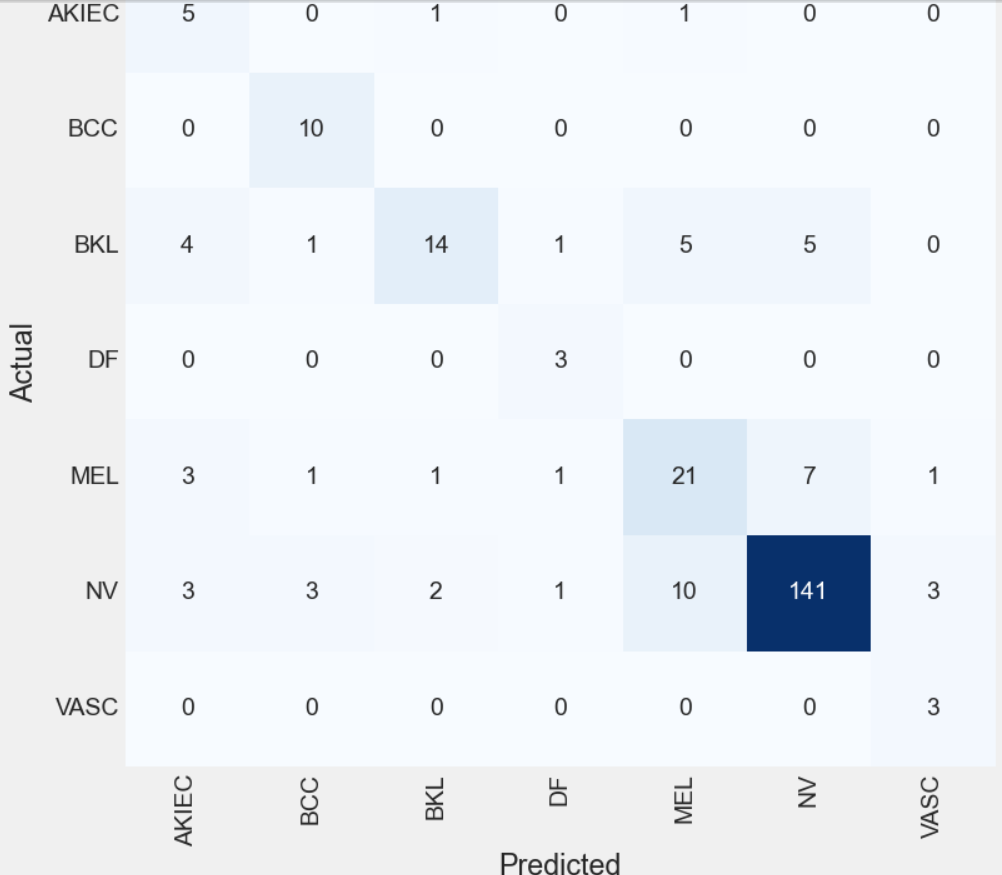
\includegraphics[width=0.45\textwidth]{./Graphics/confussion_matrix.png}
		\caption{Estadísticas de eficacia del modelo al estimar los resultados en el conjunto de pruebas.\label{fig:confussion_matrix}}
		\end{center}
		\end{figure}
    
    

%-----------------------------------------------------------------------------------
	\subsection{Estadísticas de aprendizaje}\label{sub:learning_statistics}
%-----------------------------------------------------------------------------------
		\begin{figure}[ht]%
      \begin{center}
      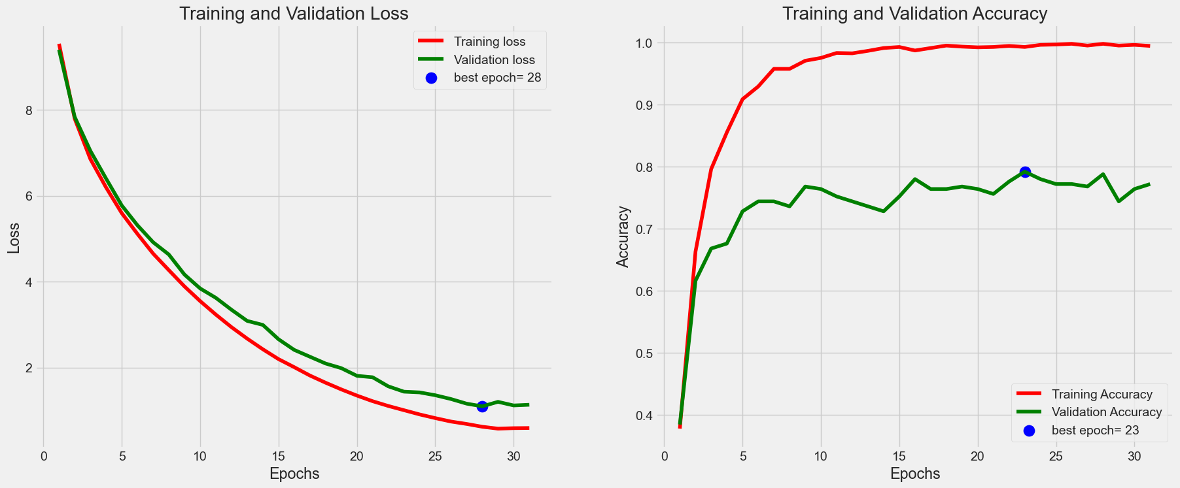
\includegraphics[width=0.45\textwidth]{./Graphics/training_validation.png}
      \caption{Estadísticas de aprendizaje a lo largo del proceso de entrenamiento (en rojo el proceso de entrenamiento en el conjunto de entrenamiento, en verde en el conjunto de validación).\label{fig:training_validation_loss}}
      \end{center}
		\end{figure}
  
La imagen anterior muestra un gráfico del curso temporal de las épocas realizadas, mostrando cómo el algoritmo iba obteniendo resultados más precisos y disminuyendo el error.

%-----------------------------------------------------------------------------------
\section{Ventajas y Desventajas}\label{sec:advantages_disadvantages}
%-----------------------------------------------------------------------------------
Las ventajas y desventajas del proceso son las siguientes. 
Ventajas: 
\begin{enumerate}
    \item Selección y representación del problema y de los datos. 
    Este proceso ayuda a comprender mejor el problema en cuestión y a identificar los datos relevantes necesarios para entrenar el modelo.
    \item Preprocesamiento de datos e imágenes. 
    Eliminar el ruido y los artefactos de las imágenes mejora la calidad de los datos y puede mejorar el rendimiento del modelo. 
    La selección de canales adecuados y la reducción del ruido también pueden mejorar el rendimiento del modelo
\end{enumerate}  
Desventajas: 	
\begin{enumerate}
    \item Modificación y procesamiento de datos. Si se utilizan conjuntos de datos inadecuados o se normalizan incorrectamente, el modelo puede no ser preciso o útil.
\end{enumerate} 



\backmatter

\begin{conclusions}
    Conclusiones
\end{conclusions}

\begin{recomendations}
    Recomendaciones
\end{recomendations}

\printbibliography[heading=bibintoc]


\end{document}